\documentclass[a4paper,12pt]{article}
\usepackage[margin=2cm]{geometry}

% Pacchetti utili di base
\usepackage[utf8]{inputenc}   % codifica dei caratteri
\usepackage[T1]{fontenc}      % font encoding
\usepackage[italian]{babel}   % lingua italiana
\usepackage{graphicx}         % immagini
\usepackage{hyperref}         % link cliccabili
\usepackage{amsmath}          % align center
\usepackage{amssymb}    % simboli matematici extra (\mathbb, \nabla, ecc.)
\usepackage{amsfonts}   % font matematici aggiuntivi
\usepackage{amsthm}     % se vuoi definire teoremi, definizioni, ecc.
\usepackage{float}       % per immagini non float
\usepackage{tikz}        % per barra sopra
\usepackage{mathcomp} % per simbolo siile al dollaro con due barre 
\usepackage{listings}

% Informazioni sul documento
\title{Linguaggi di Programmazione\\
\large Modulo II}
\author{Nicolò Giuliani}
\date{}


\begin{document}
\maketitle
\tableofcontents   % <-- genera automaticamente la pagina dell'indice
\newpage 

\section{Nomi e ambiente}
L'uso di un \textbf{nome} serve ad indicare l’oggetto denotato.
\begin{lstlisting}
const pi = 3.14;
int x;
void f(){...};
\end{lstlisting}
\textit{pi, x, f} sono nomi. Gli oggetti che denotano:
\begin{itemize}
  \item la costante 3.14
  \item una variabile
  \item la definizione di f 
\end{itemize}
Nei linguaggi i nomi sono \textbf{token} (identificatori). Il loro utilizzo serve per indicare l'\textbf{oggetto denotato}.\\
Definiamo \textbf{ambiente} ovvero l'insieme delle associazioni fra nomi e oggetti denotabile esistenti a run-time in uno specifico punto del programma ed in uno specifico momento dell’esecuzione.
Attraverso la \textbf{dichiarazione} (meccanismo col quale si) si crea un'associazione in ambiente.
\begin{lstlisting}
int x;
int f(){
  return 0;
}
type T = int;
\end{lstlisting}
Bisogna stare attenti come in diversi punti del programma lo stesso nome può essere utilizzato per oggetti diversi. Mentre attraverso \textbf{aliasing} possiamo avere nomi diversi per lo stesso oggetto (puntatori per riferimento, puntatori)
\begin{lstlisting}
int *x;
x = (int *) malloc(sizeof(int))
*x = 5;
\end{lstlisting}
Nei linguaggi moderni l'ambiente è strutturato attraverso i \textbf{blocchi}. Ovvero regioni testuali con inzio e fine che può contenere dichiarazione locali in quella regione.
\begin{lstlisting}
{
int tmp = x;
x = y;
y = tmp;
}
\end{lstlisting}
Due blocchi si sovrappongono se un blocco sta dentro un altro blocco. La dichiarazione locale è libera per un blocco annidato, a meno che una nuova dichiarazione venga fatta nel sottoblocco. \\
L'almbiente locale può essere suddiviso in 
\begin{itemize}
  \item ambiente locale: associazioni all'ingresso del blocco
  \item ambiente non locale: associazioni eridate da altri blocchi
  \item ambiente globale: parti di ambiente non locale relativo alle associazioni comuni (variabili globali, ecc)
\end{itemize}
La \textbf{vita} di un oggetto e un legame è: 
\begin{itemize}
  \item vita dell'oggeto più lunga
  \begin{lstlisting}
    fn P(int X){...} //definiamo la funzione
    int A; //definiamo la variabile
    P(A); //creiamo il legame
  \end{lstlisting}
  Durante l'esecuzione di P(A) esiste un legame tra $X$ e l'oggetto che esisteva già prima e dopo l'esecuzione della funzione.
  \item vita dell'oggetto più breve (area di memoria de-allocata)
  \begin{lstlisting}
  int *x, *y;
  x = (int *) malloc(sizeof(int));
  y = x;
  free(x);
  x=null;
  \end{lstlisting}
  Dopo la \textit{free(x)} non esiste più l'oggetto ma esiste ancora un legame per $y$ (dangling reference)
\end{itemize}
\subsection{Regole di scope}
\label{sec:scope}
Come implementiamo la regola di visibilità? \\
Una dichiarazione locale è visibile in quel blocco e in tutti i blocchi annidati, a meno di nuove dichiarazioni con stesso nome.
\begin{lstlisting}
{int x=10;
  void foo () {
    x++;
  }
  void fie (){
    int x = 0;
    foo();
  }
  fie();
}
\end{lstlisting}
Quale $x$ incrementa \textit{foo()}? Siamo in un caso di un riferimento non-locale, può essere risolto:
\begin{itemize}
  \item Scope statico (c, java, rust, ecc): nel blocco che include sintatticamente \textit{foo()}
  \begin{align*}
    x=11
  \end{align*}
  \item Scope dinamico (Emacs Lisp, perl, ecc): nel blocco che è eseguito immediatamente prima di \textit{foo()}
    \begin{align*}
    x_\text{locale} = 1 \\
    x = 10
  \end{align*}
\end{itemize}
\noindent
\begin{minipage}{0.48\textwidth}
\textbf{Scope statico}\\[2mm]
\begin{lstlisting}
{ int x=0;
void pippo(int n){
  x = n+1;
}
pippo(3);      // incrementa x globale
write(x);      // stampa x globale = 4
  {int x=0;    // ridifiniamo x locale
   pippo(3);   // incrementa x globale
   write(x);   // stampa x locale = 0
  }
write(x);      // stampa x globale = 4
}
\end{lstlisting}
Output: 404
\end{minipage}%
\hfill
\begin{minipage}{0.48\textwidth}
\textbf{Scope dinamico}\\[2mm]
\begin{lstlisting}
{ int x=0;
void pippo(int n){
  x = n+1;
}
pippo(3);      // incrementa x globale
write(x);      // stampa x globale = 4
  {int x=0;    // settiamo x locale
   pippo(3);   // incrementa x di blocco chiamante
   write(x);   // stampa x locale = 4
  }
write(x);      // stampa x globale = 4
}
\end{lstlisting}
Output: 444
\end{minipage}
\vspace{1em}\\
Per l'allocazione di memoria guarda: \nameref{sec:alloc_scope}.
\section{Memoria}
Come allochiamo la memoria?
\begin{itemize}
  \item Statica: allocazione a tempo di compilazione. \\
  Ovvero zone protette di memoria dove gli oggetti hanno indirizzi assoluti per tutta l'esecuzione. (variabili globali, costanti, ecc). Non permette la ricorsione, perche tiene  SOLO le variabili locali per sottoprogrammi).
  \begin{lstlisting}
  fn fatt(x){
    if x == 0 {
      return 1
    }
    else return x*fatt(x-1)
  }
  fatt(5):
    5*fatt(4)
  fatt(4):
    4*fatt(3)   \\ sovrascrive il vecchio x
  fatt(3):
    3*fatt(2) \\ sovrascrive ancora
  \end{lstlisting}
  Quindi sovrascrivendo sempre $x$ non possiamo mai avere un valore di ritorno valido per la ricorsione.
  \item Dinamica: allocazione a tempo di esecuzione. \\
  \begin{itemize}
    \item \textbf{Stack} (FIFO): Definiamo che ogni istanza di un sottoprogramma ha una porzione di memoria chiamato \textbf{frame stack} (record di attivazione o RdA), con le relative informazioni (anche indirizzo di ritorno di memoria). \\
      Abbiamo un puntatore \textbf{SP} (stack pointer) che punta sempre il cima allo stack, e poi abbiamo anche \textbf{FP} (frame pointer) che indica la base del frame. Così possiamo accedere a tutte le variabili con
      \begin{lstlisting}
    indirizzo = FP + offset
      \end{lstlisting}
      con FP calcolato a compile-time.\\
      \newline
      Perchè utilizziamo gli RdA e il link dinamico? Gli RdA non hanno tutti la stessa dimensione, dipende da paramatri, variabili locali, ecc, quindi il \textit{pop()} non è così semplice. Allora attraverso il link dinamico abbiamo
      \begin{center}
        \begin{lstlisting}
    | variabili locali |
    | parametri        |
    | indirizzo ritorno|
    | link_dinamico    |  \\ punta al frame precedente 
                          \\ che ci ha chiamato
        \end{lstlisting}
      \end{center}
      e quindi basta fare SP = link\_dinamico.
  \end{itemize}
  \item \textbf{Heap}: memoria nella quale i (sotto)blocchi possono essere allocati/deallocati dinamicamente arbitrariamente. \\
  Questo ci serve per gli oggetti di dimensione dinamica come stringhe, liste, alberi, puntatori, ecc. \\
  Abbiamo due modi di implementazione:
  \begin{itemize}
    \item Blocchi di memoria di dimensione fissa, li mettiamo nella \textbf{LL} (lista libera). Quando allochiamo shiftiamo il puntatore LL al primo blocco libero, mentre quando deallochiamo LL punta a quel blocco che punta al ex-primo blocco libero.
    \begin{figure}[H]
    \centering
    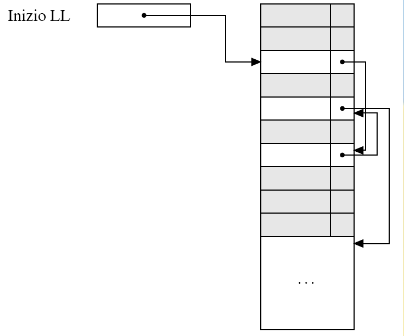
\includegraphics[width=0.5\textwidth]{img/statico.png}
\end{figure}
    \item Blocchi di memoria di dimensione variabile, partiamo con un unico blocco. Quando allochiamo prendiamo una parte del blocco di dimensione richiesta, mentre la deallocazione la restituisce alla LL. Bisogna però stare molto attenti alla frammentazione della memoria!
    \begin{itemize}
      \item Frammentazione interna: allochiamo un blocco che però è più grande di quello richesto (spreco di memoria)
      \item Frammentazione esterna: abbiamo abbastanza spazi sparsi ma separati
    \end{itemize}
  \end{itemize}
    Come gestiamo quindi la LL unica? Ad ogni allocazione possiamo fare:
    \begin{itemize}
      \item first fit: primo blocco abbastanza grande
      \item best fit: minor blocco abbastanza grande
    \end{itemize}
  Possiamo migliorare? Attraverso LL multiple (blocchi dimensione variabile). Però come ripartiamo i blocchi fra le LL?
  \begin{itemize}
    \item statica
    \item dinamica
  \end{itemize}
\end{itemize}
\subsection{Implementazione delle regole di \hyperref[sec:scope]{scope}}
\label{sec:alloc_scope}
\begin{itemize}
  \item Scope statico
  \begin{itemize}
    \item Catena statica \\
    Immaginiamo di Avere 
    \begin{center}
    main $\to$ A $\to$ B $\to$ C $\to$ D $\to$ E $\to$ C
    \end{center}
     
  \begin{minipage}{0.48\textwidth}
     \begin{figure}[H]
    \centering
    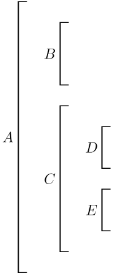
\includegraphics[width=0.3\textwidth]{img/catena.png}
    \end{figure}
  \end{minipage}%
  \hfill
  \begin{minipage}{0.48\textwidth}
       \begin{figure}[H]
    \centering
    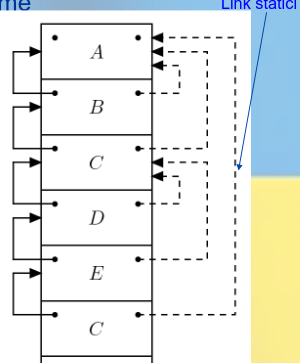
\includegraphics[width=0.7\textwidth]{img/statici.png}
    \end{figure}
  \end{minipage}
  Se un sottoprogramma è a livello $k$ implica che la catena è lunga $k$.\\
  Se $k=0$ il chiamante punta SP alla funzione, se $k>0$ il chiamante risale la catena $k$-volte. Ogni volta che incontriamo un nome ci segniamo se è locale con $h=0$ o se era stato definito $h$-blocchi fa.
    \item Display\\
    Possiamo ottimizzare il costo $h$ per la lettura di un nome non locale attraverso un array con $i$ RdA attivo definito ad RdA $i-1$. Così possiamo trovare la posizione di un oggetto con $i-h$. Quando aumentiamo la catena $k+1$ il chiamante e il processo non condividono più il $Display[k+1]$.\\
    Nella realtà il dispay è più costoso nella sequenza di chiamate e quindi è poco utilizzato.
  \end{itemize}
  \item Scope dinamico
  \begin{itemize}
    \item A-list\\
    Le associazioni sono memorizzate in una struttura apposita, manipolata come una pila.
    \item CRT (Tabella centrale dell'ambiente)\\
    Una tabella mantiene tutti i nomi distinti del programma. Se i nomi sono noti il costo è costante, se no costo hash.
  \end{itemize}
\end{itemize}
\section{Controllo}
Come strutturiamo il controllo del flusso di un linguaggio?
\subsection{Espressioni}
Entità sintattica che produce un valore o è indefinita. La sintassi può essere
\begin{itemize}
  \item Infissa: $a+b$\\
  Gli operatori aritmetici hanno precedenza su contronto che hanno a loro volta precedenza su logici. Le parentesi sono essenziali in alcuni casi. L'associatività dipende dal tipo di operando.
  \item Prefissa: $+ab$\\
  Si valuta attraverso una pila, si legge il prossimo simbolo e lo si mette sulla pila, se abbiamo un operatore applichiamo l'operazione su i valori della pila prima del operatore e lo memorizziamo $R$. Eliminiamo operatore e operandi, memorizziamo $R$ in pila.
  \item Postfissa: $ab+$\\
  Sempre attraverso una pila ma dobbiamo contare gli operandi che vengono letti
\end{itemize}
    \begin{figure}[H]
    \centering
    
\includegraphics[width=0.2\textwidth]{img/albero.png}
\end{figure}
Le espressioni possono essere rappresentate come alberi, a seconda del tipo di visita di albero abbiamo una delle 3 precedenti notazioni lineare. A partire dall’albero il compilatore produce il codice oggetto oppure l’interprete valuta l’espressione. \\
Ovviamente la valutazione può comportare dei risultati diversi (effetti collaterali)
\begin{lstlisting}
(a+f(b)) * (c+f(b))
\end{lstlisting}
Se $f(b)$ modifica $b$ allora il risultato da sinistra a destra è diverso di quello da destra a sinistra.\\
\subsection{Comandi}
Un comando è un’ entità sintattica la cui valutazione non necessariamente restituisce un valore, ma può avere un effetto collaterale. \\
Sapendo che una \textbf{variabile} è un "contenitore" modificabile di valori con un nome. Attraverso il comando di assegnamento possiamo modificare il valore di una variabile.
\begin{lstlisting}
x := 2
x = x+1
\end{lstlisting}
Il primo $x$ è un l-value ovvero una locazione, mentre il secondo $x$ è un r-value ossia un valore che può essere contenuto in una locazione. Anche la assegnazione comporta effetti collaterali (anche se non ritorna un valore sempre).
\begin{lstlisting}
//C
x = 2; //ritorna 2
y = x = 2; //valido
\end{lstlisting}
Questo vale un po' per tutti i linguaggi imperativi. Mentre nei linguaggi funzionali (Haskell, ecc) assomiglia più al modello matematico, una variabile denota un valore ed è immutabile. I linguaggi logici danno la possibilità di modifica entro certi limiti.\\
Abbiamo anche il \textbf{modello a riferimento}, ovvero una variabile è riferimento ad un valore che ha un nome
\begin{lstlisting}
x --> 2
\end{lstlisting}
Simile ai puntatori, ma i puntatori hanno le allocazioni esplicite.\\
    \begin{figure}[H]
    \centering
    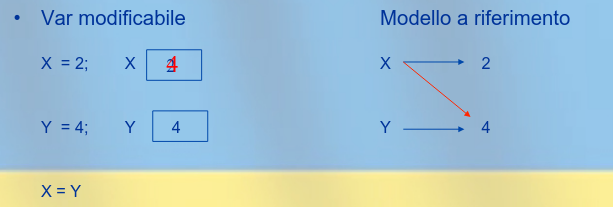
\includegraphics[width=0.5\textwidth]{img/rif.png}
\end{figure}
\vspace{3em}
\subsection*{Ambiente e memoria}: Due variabili diverse possono denotare lo stesso oggetto? Nomi ---> Valori non basta!\\
Nei linguaggi imperativi abbiamo
\begin{itemize}
  \item Valori Denotabili (quelli che possono dare i nomi)
  \item Valori Memorizzabili (quelli che si pososno memorizzare)
  \item Valori Esprimibili (risultato della valutazione di una exp.)
\end{itemize}
Come gestiamo i \textbf{comandi per il controllo sequenza}? \\
\textbf{Esplicitamente} con ";", "blocchi" o "goto", ma non bastano per la \textit{programmazione strutturata}. \textbf{Comandi condizionali} come "if case" o comandi iterativi "for while". Questi ultimi 2 comandi permettono di avere codice ben strutturato e non "spaghetti code". Questi pemettono una maggiore leggibilità e anche ottimizzazione se compilato in modo astuto. \\
\vspace{1px}\\
Come sappiamo Iterazione e ricorsione sono i due meccanismi che permettono di ottenere formalismi di calcolo Turing completi. Senza di essi avremmo automi a stati finiti.
\subsubsection{Iterazione}
Abbia due tipologie di iterazione
\begin{itemize}
  \item indeterminata: cicli controllati logicamente, non noto a priori al avvio del ciclo (while, repeat, ecc). Questo è il vero potere delle MdT. Si implementano attraverso l’istruzione di salto condizionato della macchina fisica.
  \item determinata: cicli controllati numericamente, ovvero noto a priori (do, for, ecc)
\end{itemize}
\subsection{Ricorsione}
Modo alternativo all’iterazione per ottenere il potere espressivo delle MdT. \\
La definizione di una funzione ricorsiva è analoga alla definizione induttiva di una funzione. Ogni programma iterativo può essere riscritto in ricorsivo e viceversa.\\
In caso di implementazioni naif ricorsione meno efficiente di iterazione possiamo utilizzare optimizing compiler che produce codice efficiente o tail-recursion.\\
La ricorsione in coda (tail recursion): Una chiamata di g in f di si dice “chiamata in coda” (o tail call) se f restituisce il valore restituito da g senza ulteriore computazione.
\begin{lstlisting}
function tail_rec (n: integer): integer
  begin ... ; x:= tail_rec(n-1) end
function non_tail rec (n: integer): integer
  begin ... ; x:= non_tail_rec(n-1); y:= g(x) end
\end{lstlisting}
Qui la chiamata ricorsiva è l’ultima operazione eseguita dalla funzione, la funzione ritorna direttamente il risultato della chiamata ricorsiva. Dopo \textit{tail\_rec(n-1)} non c’è più nulla da fare.\\
Non serve allocazione dinamica della memoria con pila: basta un unico RdA.
\begin{figure}[H]
    \centering
    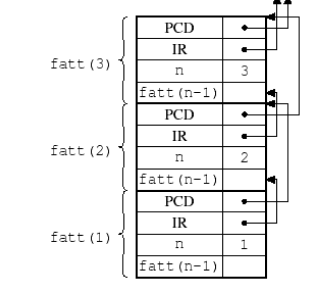
\includegraphics[width=0.3\textwidth]{img/fatt.png}
\end{figure}
Possibile la generazione di codice tail-recursive usando continuation passing style (passare il resto come parametro), questo rende più efficiente il costo computazionale e di spazio.1
\begin{figure}[H]
    \centering
    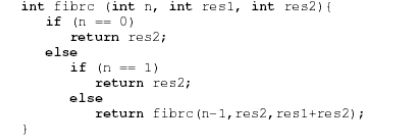
\includegraphics[width=0.5\textwidth]{img/fib.png}
\end{figure}
Costo lineare di tempo $n$ e spazio costante (1 RdA).
\section{Sottoprogrammi}
I LP sono essi stessi astrazioni del calcolatore sottostante.
\begin{center}
  LP alto livello $\iff$ maggiore astrazione
\end{center}
\begin{itemize}
  \item Astrazione sul controllo: fornisce astrazione funzionale al progetto (comunica con parametri, ambiente globale)
  \begin{figure}[H]
    \centering
    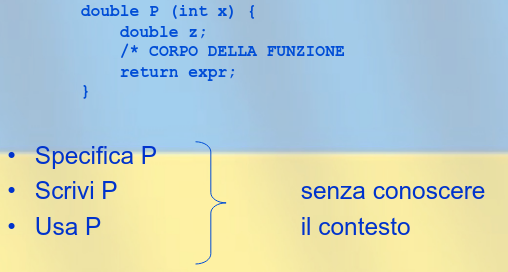
\includegraphics[width=0.5\textwidth]{img/controllo.png}
\end{figure}
  \item Atrazione sui dati: implementazione dei dati/operazioni inaccessibile all'utente
\end{itemize}
\subsection{Parametri}
  \begin{figure}[H]
    \centering
    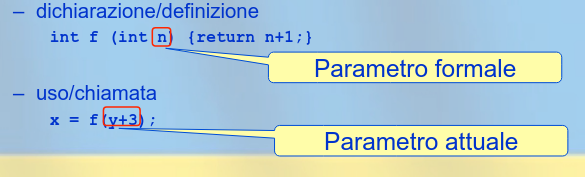
\includegraphics[width=0.5\textwidth]{img/term.png}
\end{figure}
Come passiamo i parametri?
\begin{itemize}
  \item per valore: il valore dell’attuale è assegnato al formale, che si comporta come una variabile locale
  \item per riferimento: è passato un riferimento (indirizzo) all’attuale; i riferimenti al formale sono riferimenti all’attuale (\textit{aliasing})
  \item per costante (read-only): nella procedura non è permessa la modifica del formale
  \item per risultato
    \begin{figure}[H]
    \centering
    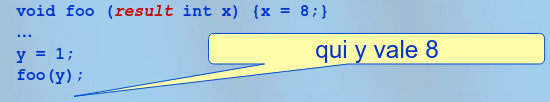
\includegraphics[width=0.5\textwidth]{img/risultato.png}
\end{figure}
  \item per valore/risultato
      \begin{figure}[H]
    \centering
    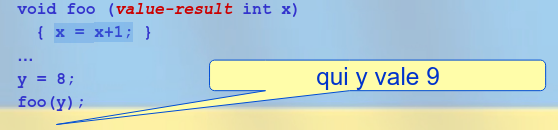
\includegraphics[width=0.5\textwidth]{img/vrisultato.png}
\end{figure}
  \item per nome: una chiamata di $P$ è la stessa cosa di eseguire il corpo di $P$ dopo aver sostituito i parametri attuali al posto dei parametri formali
        \begin{figure}[H]
    \centering
    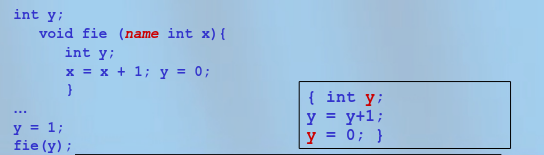
\includegraphics[width=0.5\textwidth]{img/nome.png}
\end{figure}
  Può portare conflitti di nomi!
\end{itemize}
\vspace{2em}
Alcune funzioni permettono di passare come parametro altre funzioni (puntatore al RdA all’interno della pila). O magari restituire delle funzioni (mantenere il RdA della funzione restituita, la pila non va più bene). Come gestire l’ambiente della funzione?\\
\begin{lstlisting}
int x=4; int z=0;
int f (int y){
  return x*y;}
void g ( int h(int n) ) {
  int x;
  x = 7;
  z = h(3) + x ;
  end;}
...
{ int x = 5;
  g(f);
}
\end{lstlisting}
Quale $x$ utilizziamo in $f$?
\begin{itemize}
  \item scope statico: la $x$ esterna
  \item scope dinamico: ha senso sia la $x$ del blocco di chiamata che la $x$ interna
\end{itemize}
\subsection{Downward funarg problem}
Quando una procedura viene passata come parametro, si crea un riferimento tra un nome (par formale: $h$) e una procedura (par attuale: $f$).\\
Ovvero: Quale ambiente non locale si applica al momento dell’esecuzione di $f$ (in quanto chiamata via $h$)?
\begin{itemize}
  \item \textbf{Deep binding}: ambiente al momento della creazione del legame $h \to f$ (scope statico)
  \item \textbf{Shallow binding}: ambiente al momento della chiamata di $f$ via $h$ (forse scope dinamico)
\end{itemize}
        \begin{figure}[H]
    \centering
    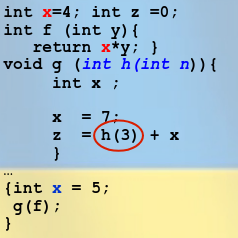
\includegraphics[width=0.3\textwidth]{img/scope.png}
\end{figure}
\begin{itemize}
  \item Scope statico: 
  \begin{itemize}
    \item Deep: $x$ rossa (esterna)
    \item Shallow: $x$ rossa (esterna)
  \end{itemize}
  \item Scope dinamico:
    \begin{itemize}
    \item Deep: $x$ azzurra (blocco di chiamata)
    \item Shallow: $x$ nera (blocco interno)
  \end{itemize}
\end{itemize}
\paragraph{Passare una chiusura} Passare dinamicamente sia il legame col codice della funzione, che il suo ambiente non locale,cioè una chiusura $<code, \, env>$.\\
Quindi allochiamo (come sempre) RdA, prendiamo il puntatore di catena statica dalla chiusura.\\
\vspace{1px}\\
Come li implementiamo?
\begin{itemize}
  \item Scope statico
    \begin{itemize}
    \item (SEMPRE) Deep: implementato con chiusure
    \item Shallow: non si fa, ma non fa differenza con deep
  \end{itemize}
  \item Scope dinamico
  \begin{itemize}
    \item Deep: usa necessariamente qualche forma di chiusura per “congelare” uno scope da riattivare più tardi
    \item Shallow: per accedere ad $x$ risali la pila (A-list, CRT)
  \end{itemize}
\end{itemize}
\subsection{Upward funarg problem}
Alcuni linguaggi (eg funzionali) permettono di restituire una funzione. Se la funzione ha variabili locali queste devono sopravvivere indipendentemente dalla struttura a pila: hanno vita indefinitamente lunga.
        \begin{figure}[H]
    \centering
    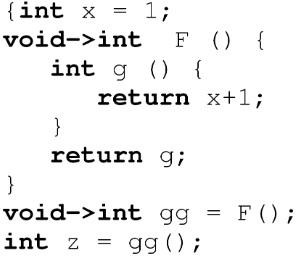
\includegraphics[width=0.2\textwidth]{img/up.png}
\end{figure}
$F$ ritorna una chiusura.\\
\vspace{1px}\\
La pila (LIFO) non va più bene, come implementiamo la "pila" corretta?
\begin{itemize}
  \item non deallocare esplicitamente
  \item record di attivazione sullo heap
  \item le catene statica e dinamica collegano i record
  \item invoca il garbage collector quando necessario
\end{itemize}
\subsection{Eccezioni}
Terminare parte di una computazione quando richiesto e gestire l'eccezione se sorta.
        \begin{figure}[H]
    \centering
    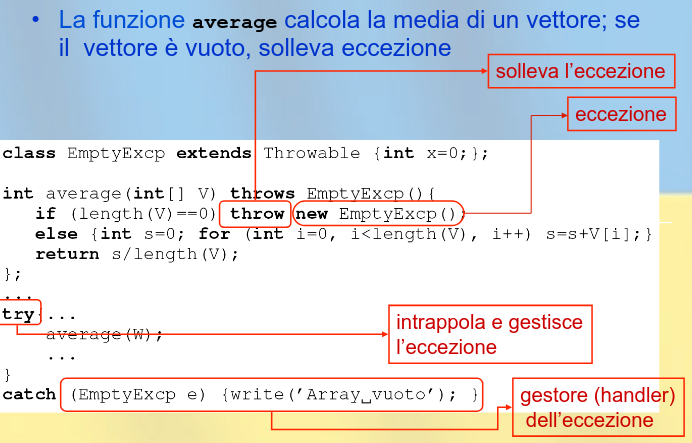
\includegraphics[width=0.7\textwidth]{img/ec.png}
\end{figure}
Il gestore è legato in modo statico al blocco di codice protetto, l’esecuzione del gestore rimpiazza la parte di blocco che doveva essere ancora eseguita.\\
\vspace{1px}\\
Possiamo anche utilizzare le eccezioni per rendere più efficiente un codice:\\
Problema: Calcolare il prodotto tra tutti i nodi di un albero
\begin{itemize}
  \item NON OTTIMIZZATA:
    \begin{lstlisting}
      int mul(T tree){
       if (tree == null) return 1;
       return tree.value * mul(tree.L) * mul(tree.R);
      }
    \end{lstlisting}
  \item OTTIMIZZATA:
  \begin{lstlisting}
    int mulAus(T tree){
       if (tree == null) return 1;
       if (tree.value == 0) {
        throw new Zero();
       }
       return tree.value * mul(tree.L) * mul(tree.R);
    }
  
    int mul(T tree){
      try{
      return mulAus(tree)
      } catch (Zero e){
        return 0;
      }
    }
  \end{lstlisting}
\end{itemize}
\vspace{2em}
\paragraph{Come implementiamo le eccezioni?} 
Il compilatore genera una \emph{tabella delle eccezioni} che, per ogni blocco
protetto (\texttt{try}), contiene una coppia del tipo
\[
\langle \mathit{block\_addr}, \mathit{handler\_addr} \rangle
\]
(dove in realtà il blocco è identificato da un intervallo di indirizzi).

La tabella è ordinata staticamente rispetto a $\mathit{block\_addr}$.

Quando viene sollevata un’eccezione, il runtime prende l’indirizzo corrente
di esecuzione (Program Counter) e cerca nella tabella il blocco che lo contiene,
tipicamente tramite \emph{ricerca binaria}.

Una volta individuata la voce corrispondente, il controllo viene trasferito
all’indirizzo del gestore ($\mathit{handler\_addr}$), dopo aver effettuato lo
\emph{stack unwinding}.

Se il gestore rilancia l’eccezione, il processo viene ripetuto nel frame
chiamante, continuando la ricerca di un gestore compatibile. Se non lo trova il programma finisce senza gestire l'eccezione.
\end{document}


